%!TEX root = ../thesis.tex

\section{Introduction}

In sports, dance performance, and body gesture interfaces, movement instructions are often conveyed with drawings of the human body annotated with arrows or stroboscopic effects~\cite{cutting_representing_2002} (see Figure~\ref{fig:existing_examples} for examples).
These \textit{illustrations of human movements} are also used within HCI to convey new user experiences in papers and storyboards~\cite{Buxton:2007:SUE:1526229}.
When designed well, these illustrations can precisely depict the direction of motion while excluding unnecessary details such as clothing and backgrounds~\cite{cutting_representing_2002}.

\begin{figure}[t]
  \centering
  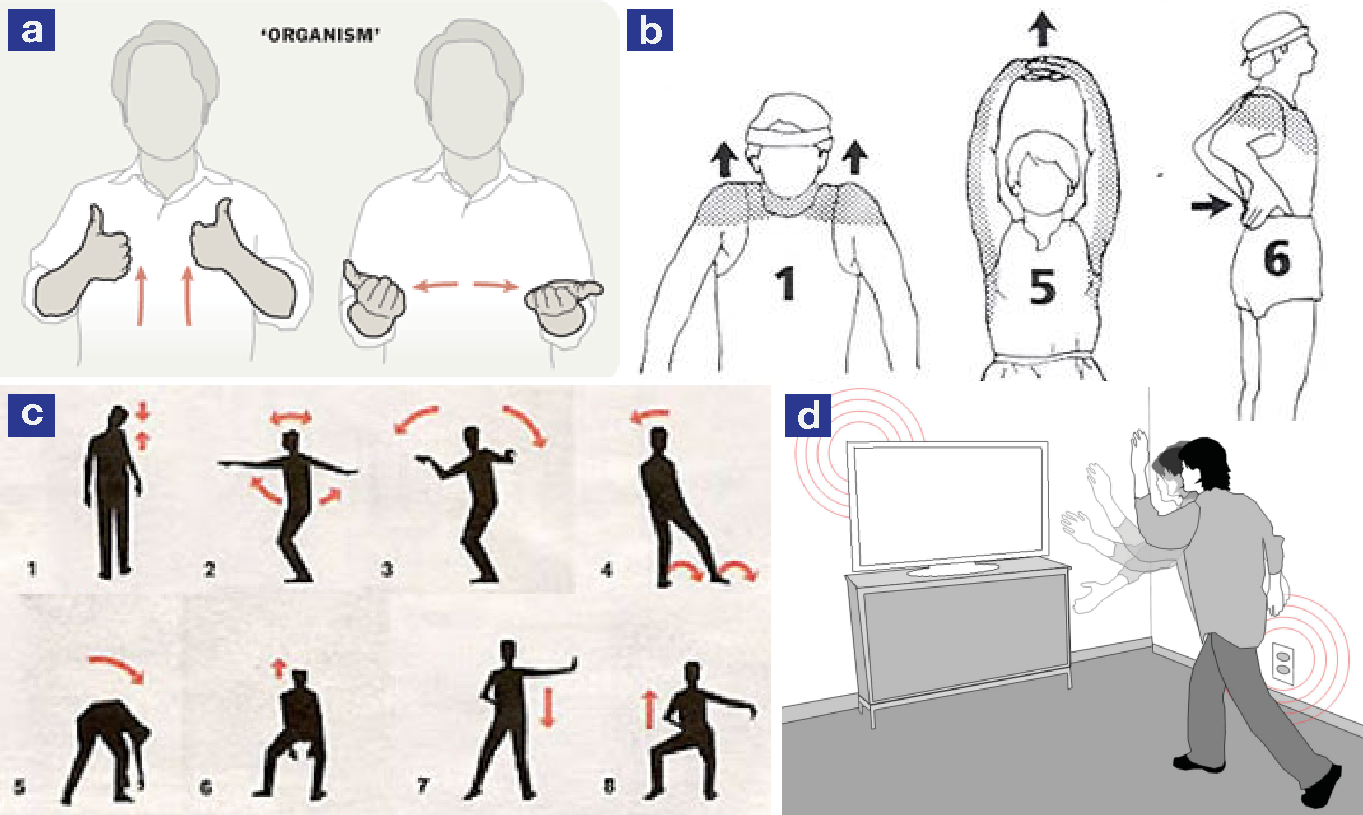
\includegraphics[width=0.7\columnwidth]{\demodraw/fig/existing_examples/existing_examples}
  \caption{Examples of manually generated human movement illustrations: (a) for sign language~\protect\cite{corum:2012:sign}; (b) for weight training~\protect\cite{anderson2010stretching}; (c) for dance steps [unknown]); (d) for a gestural interface~\protect\cite{cohn2012humantenna}.}
  \label{fig:existing_examples}
\end{figure}

We found that both professionals and non-designers create these kinds of illustrations, but the methods they use are commonly time-consuming and not amenable to iteration and editing.
The typical workflow is to prepare the physical scene, pose and photograph actors, and create annotated illustrations from the source photos. Even with the photos, producing effective depictions of the actors with integrated motion arrows and/or stroboscopic overlays takes considerable time and skill. Overall, the entire authoring process can take from 10 minutes up to several hours. Moreover, it can be difficult to identify the appropriate pose and viewpoint for the source photos before seeing the resulting illustrations.
%
For example, one may choose to exaggerate or change the orientation of a hand gesture after seeing the illustrated motion.
%
Unfortunately, making such adjustments often requires starting over again with new source photos.

To address these challenges, we propose \systemname{}, a system that enables authors to rapidly create step-by-step motion illustrations through physical demonstration (see Figure~\ref{fig:demodraw_teaser}). DemoDraw offers two key advantages over existing workflows. First, our system automatically renders characters and motion arrows based on demonstrations, which significantly reduces the amount of time and effort required to create an illustration. Second, DemoDraw helps users iteratively refine demonstrations to produce effective depictions. In our system, users can quickly add, replace, preview and modify demonstration takes.

Authoring proceeds in two modes: {\em Demonstration}, performed using body motions and voice commands; and {\em Refinement}, which uses a desktop interface.
%
The user first physically demonstrates desired motions in front of a Kinect RGB-D sensor. As in current instructional practice, they simultaneously speak during important parts (e.g., teaching dance moves with ``one, two, three, four'').
The motions are then mapped to a 3D human avatar rendered as a black-and-white contour drawing, a common style identified in our survey of illustration practices.
%
An algorithm analyzes speech and motion streams to segment motions into illustration figures with key frames. Salient joint movements are automatically identified and rendered as motion arrows overlaid on the stylized body drawing (Figure~\ref{fig:DemoDrawUI}c).
%
With this {\em \phaseI{}}, segmented motions can be reviewed and re-recorded using speech commands.
In addition, the annotation style and placement can be adjusted, camera angles moved, and alternate visualization styles explored in a mouse-driven GUI \emph{\phaseII{}} (see Figure~\ref{fig:DemoDrawRefinementUI}a).
%
A three-part evaluation with 14 participants shows that \systemname{}'s illustrations are effective and amateur authors can use the \phaseI{} and \phaseII{} to proficiently create motion illustrations with various levels of complexity.

\begin{figure*}[t!]
  \centering
  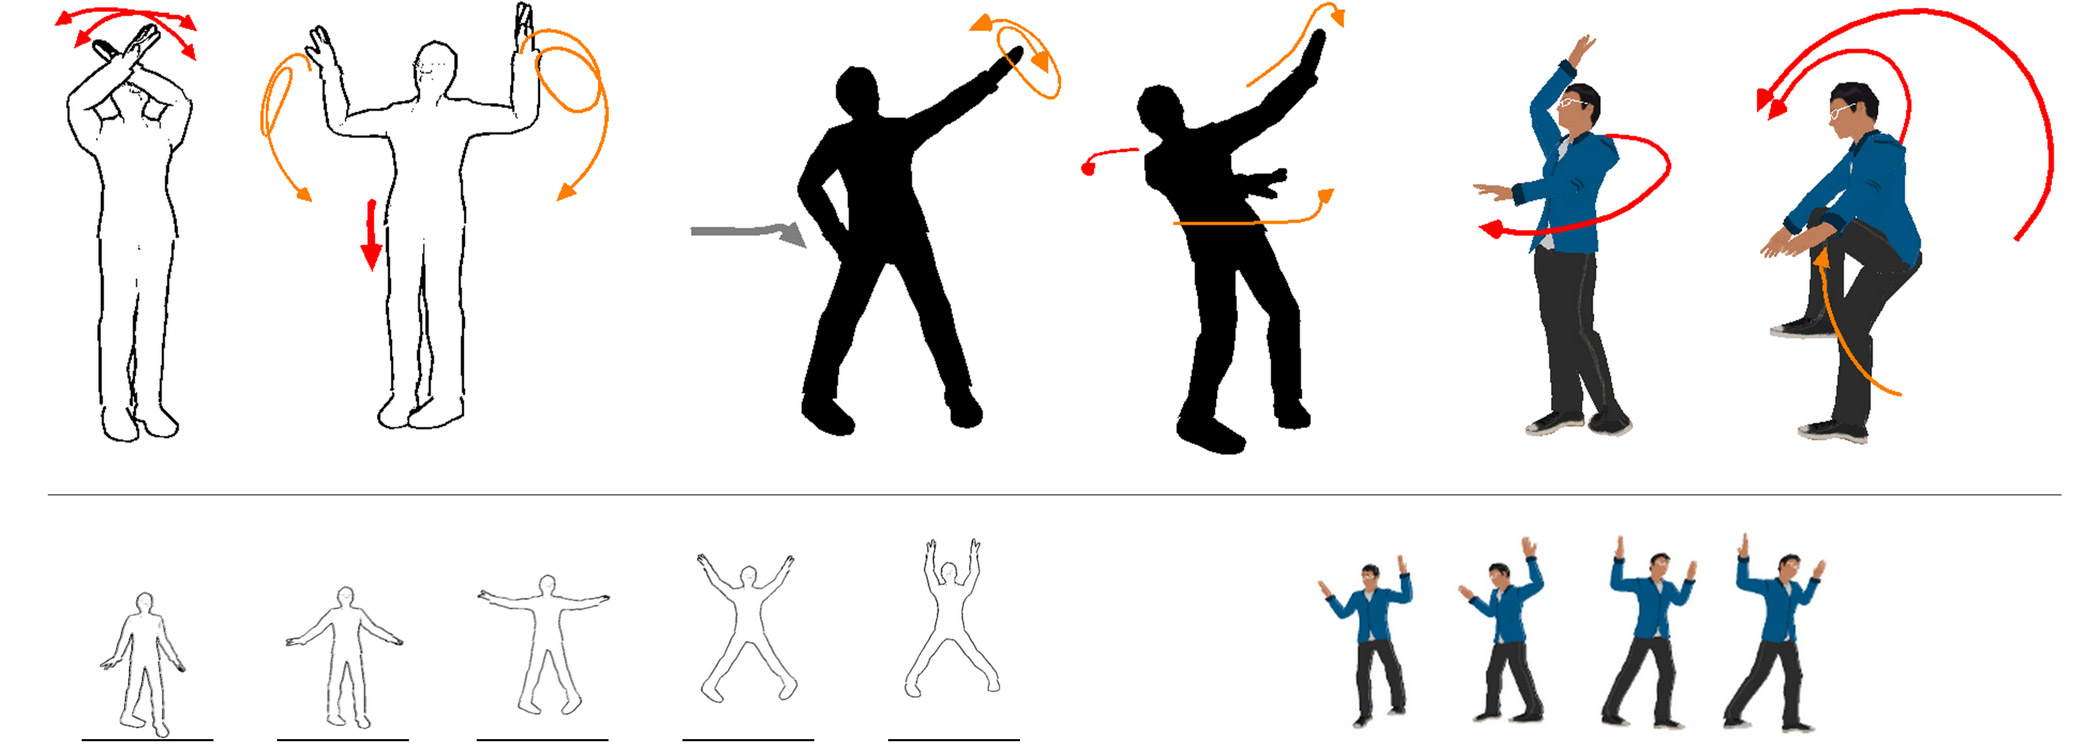
\includegraphics[width=0.8\textwidth]{\demodraw/fig/teaser/teaser}
  \caption{\systemname{}'s authoring interfaces and results: (a) multi-modal \textit{\phaseI{}} to capture motion, verify results, and re-perform portions if needed; (b) conventional \textit{\phaseII{}} for refinement and exploring other visualization styles; (c-d) examples of illustration styles (annotated with camera viewing angle $\theta$, motion arrow offsets $\delta$, stroboscopic overlap ratio $\rho$, and numbers of intermediate frames $n$).}
  \label{fig:demodraw_teaser}
\end{figure*}

DemoDraw integrates physical demonstration and authoring into one interactive workflow. Our work is the first to generate human movement illustrations by demonstration, refinement, and editing as an iterative process. %Specifically, we make the following contributions:
Our work includes the following specific contributions:

\begin{itemize}
  \item An approach to generate human movement illustrations by direct physical demonstration and interactive rendering.
  \item Multi-modal interaction techniques to record, review, retake, and refine demonstration sequences.
  \item Methods to automatically analyze 3D motion data with speech to generate step-by-step annotated illustrations.
\end{itemize}

% \clearpage
